\section{Dashboard}
\label{sec:dashboard}

KSA dashboard is, perhaps, the most complex component of all. We are using NextJS framework for the development. The application's code is broken down into 10 custom ReactJS components and defines 8 new types. We mostly use client components, only the API components run on the server side of the NodeJS application. The whole user experience is based on the \lstinline{useEffect} and \lstinline{useState} React functions, that reload data from the backend upon changes in the selected filters or search query. Additionally, community-made Lucide React icons are used to enhance user experience.

Figure~\ref{img:ksa-dashboard-ui} displays the dashboard interface. Top side of the dashboard is reserved for the filters, action buttons and search panel. Upon selecting the scanner and item type (Vulnerability or Misconfiguration), user are able to choose from the available reports to load the items. When ``All scanners'' is selected, dashboard fetches and displays misconfigurations or vulnerabilites from the latest reports (if such exist) generated by all scanners. First button on the action bar triggers a new scan for the selected scanner. Second button allows to download a JSON report, which includes all of the displayed items. Third and fourth buttons delete or resolve all of the filtered items, respectively. That is, users are able to filter items by a keyword and then delete or resolve all of them at once. This is very useful when, for instance, we are bound by a specific Java version by the contract with the customer. Therefore, we, perhaps, would want to mark all of the vulnerabilites which are filtered by the ``Java'' keyword as resolved.

\begin{figure}[!hbt]
	\begin{center}
		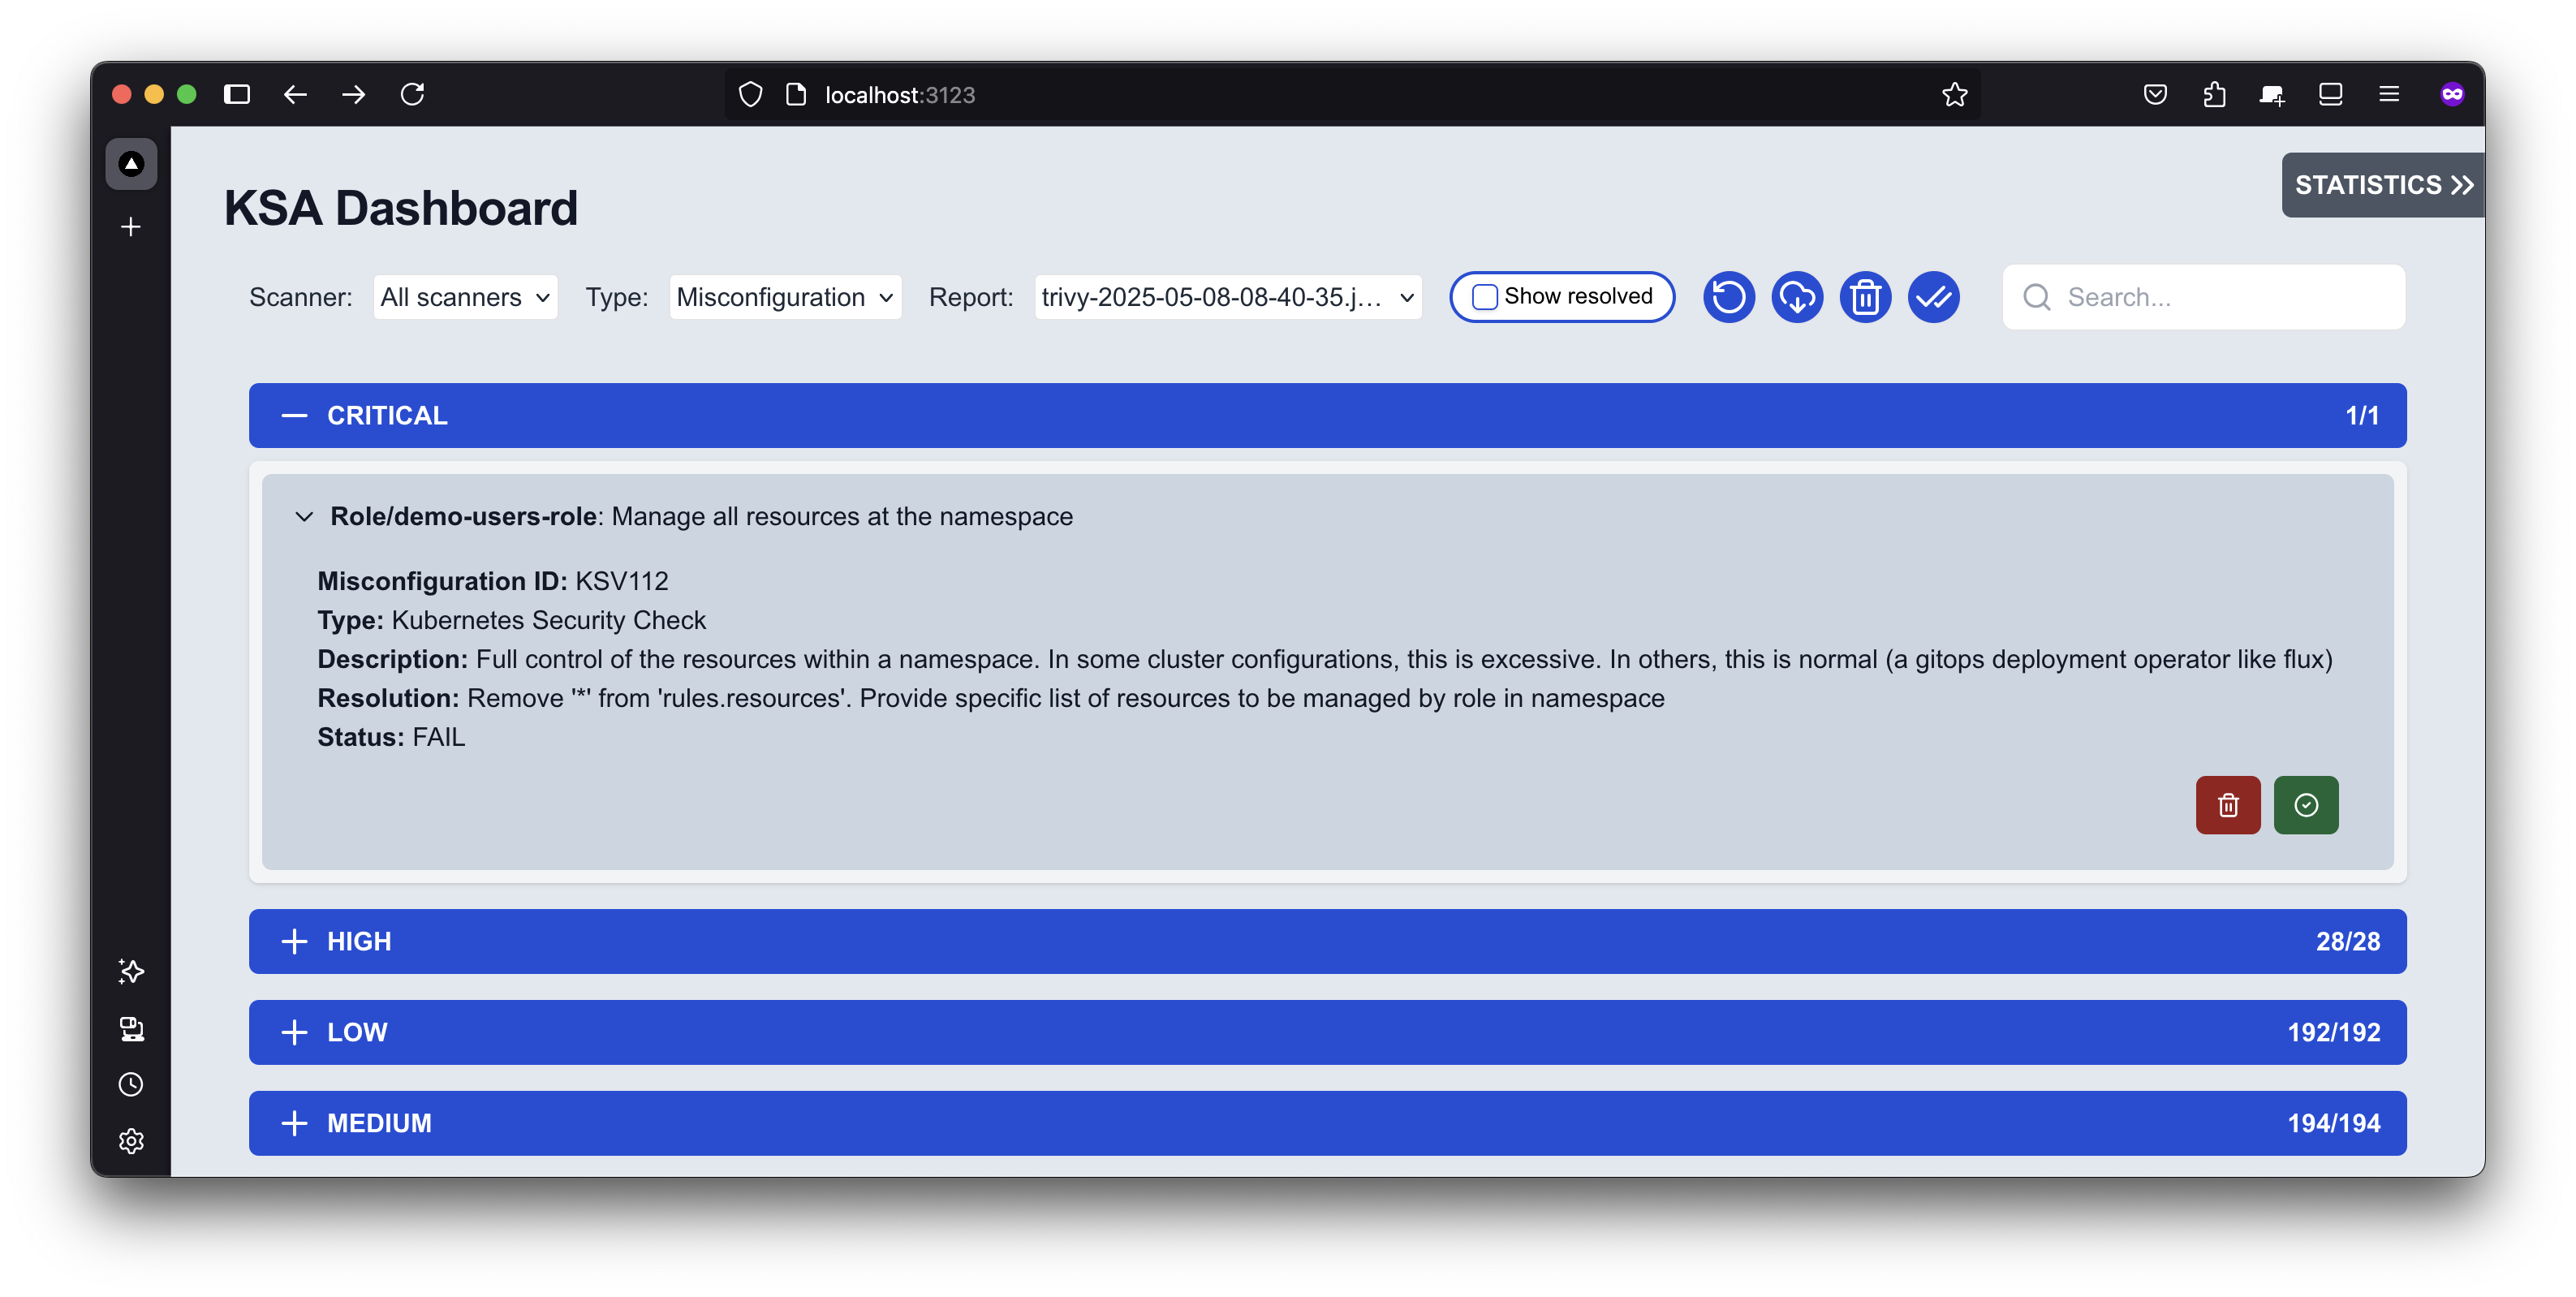
\includegraphics[width=0.9\textwidth]{images/ksa-dashboard-ui.png}
        \caption{User interface of the KSA dashboard.}
		\label{img:ksa-dashboard-ui}
	\end{center}
\end{figure}

The space below the panel is occupied by the list of the security threats. They are collapsed under different categories. Each item can be then also opened to examine the details, such as misconfiguration identifier, type, description, resolution and status. Item titles usually also include the target resource, where the misconfiguration was found.

In the top right corner of the dashboard is a \textbf{STATISTICS} button that provides some information on the most recent scan results in graphical format as shown below in Fig~\ref{img:ksa-dashboard-statistics}.

\begin{figure}[!hbt]
	\begin{center}
		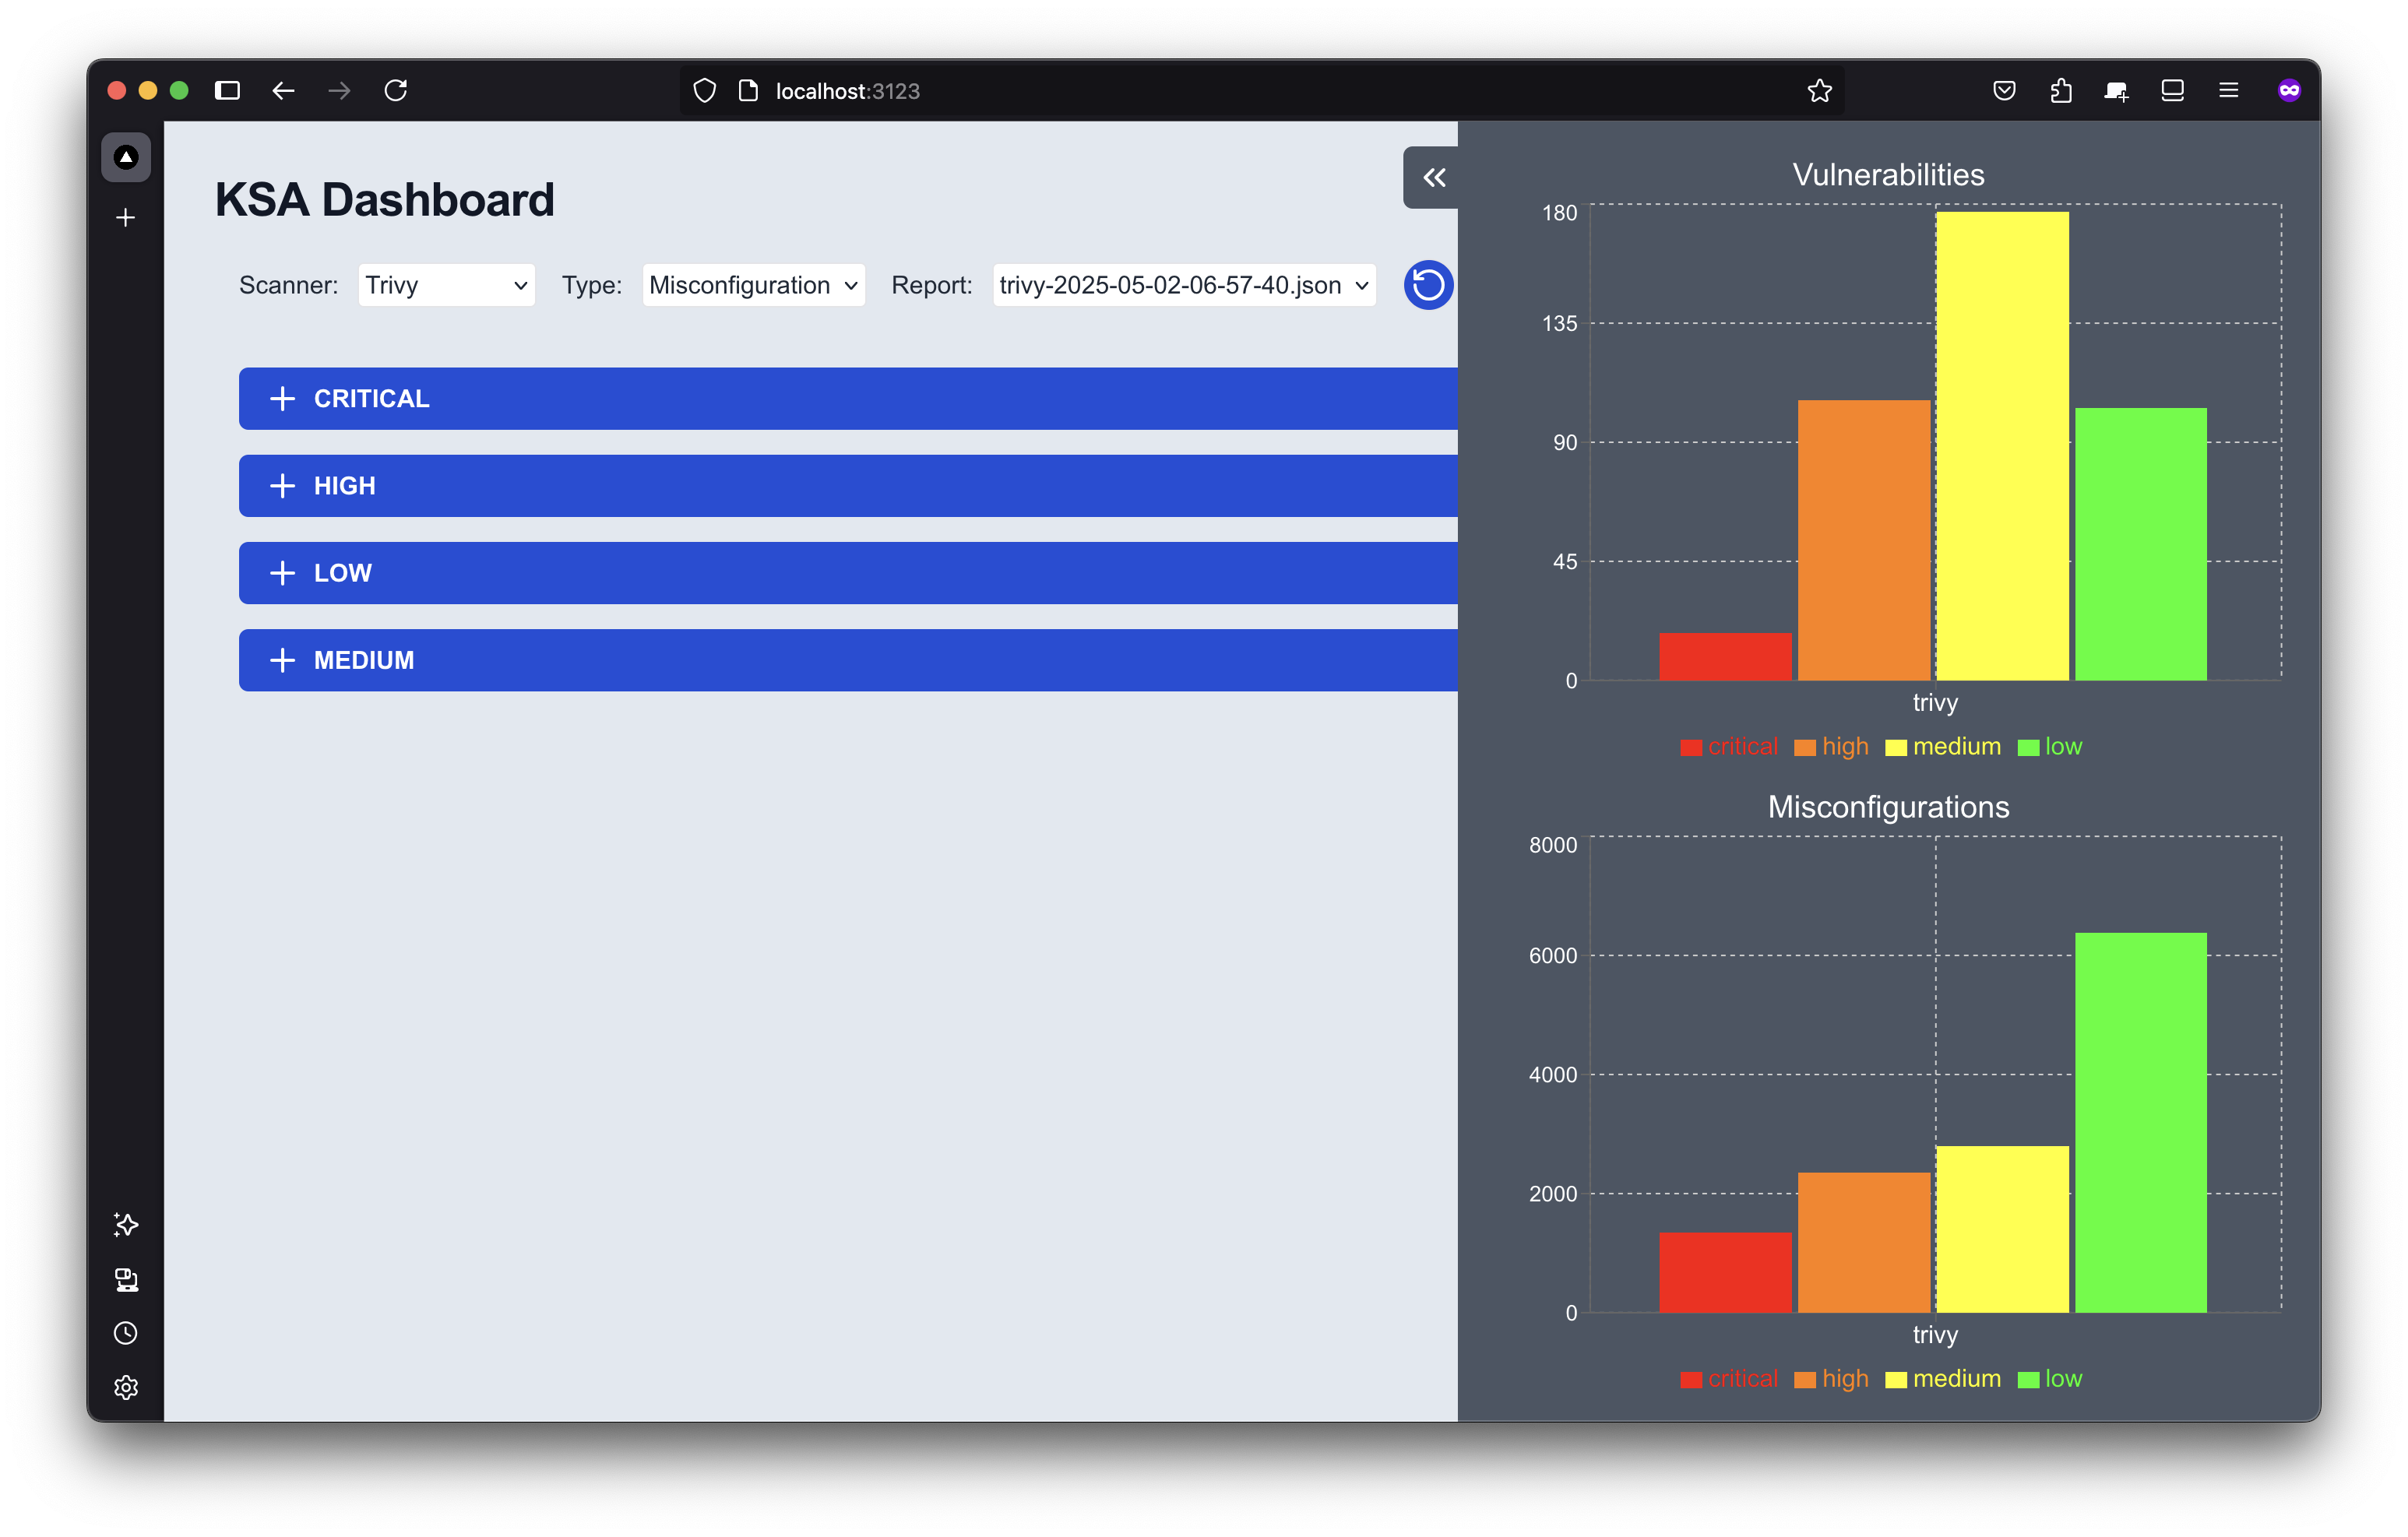
\includegraphics[width=0.9\textwidth]{images/ksa-dashboard-statistics.png}
        \caption{Statistics on the KSA dashboard.}
		\label{img:ksa-dashboard-statistics}
	\end{center}
\end{figure}